\documentclass{article}
\usepackage{fontspec}
\usepackage{siunitx}
\usepackage{tikz}
\usetikzlibrary{shapes,arrows.meta,positioning,calc,automata,mindmap}
\usepackage{circuitikz}
\usepackage{pgfplots}
\pgfplotsset{compat=1.18}
\usepackage{chemfig}
\usepackage{mhchem}
\usepackage{tikz-3dplot}
\usepackage[compat=1.1.0]{tikz-feynman}
\usepackage{tikz-cd}
\usepackage{forest}
\usepackage{tikz-timing}
\usepackage{bytefield}
\usepackage{pgfgantt}
\usepackage{tikz-dimline}
\usepackage{tikzscale}
\usepackage{endleaf-floorplan}
\begin{document}
\qty{1}{\metre}
\begin{circuitikz}
  \draw (0,0) to[R] (2,0);
\end{circuitikz}

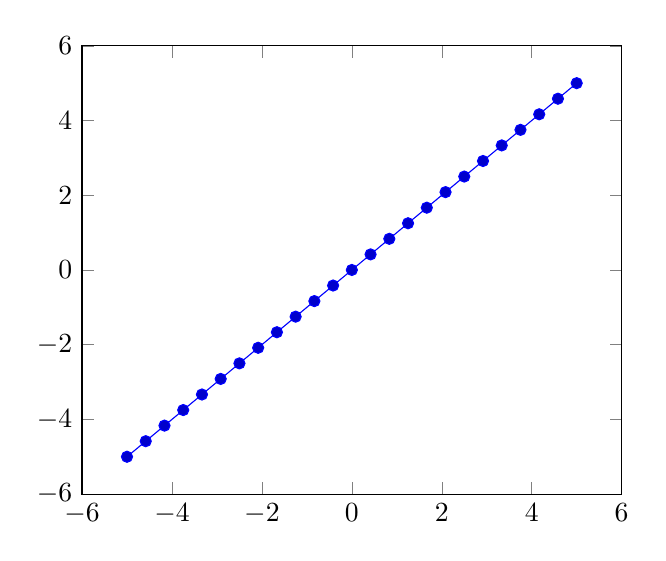
\begin{tikzpicture}
  \begin{axis}
    \addplot {x};
  \end{axis}
\end{tikzpicture}

\chemfig{H-O-H}
\ce{H2O}

\tdplotsetmaincoords{70}{110}
\begin{tikzpicture}[tdplot_main_coords]
  \draw[->] (0,0,0) -- (1,0,0);
\end{tikzpicture}

\begin{tikzpicture}
  \begin{feynman}
    \vertex (a);
    \vertex [right=of a] (b);
    \diagram* {(a) -- (b)};
  \end{feynman}
\end{tikzpicture}

\begin{tikzcd}
  A \arrow[r] & B
\end{tikzcd}

\begin{forest}
  [A [B] [C]]
\end{forest}

\texttiming{HL}

\begin{bytefield}{8}
  \bitheader{0-7}\\
  \bitbox{8}{op}
\end{bytefield}

\begin{ganttchart}{1}{2}
  \ganttbar{Task}{1}{2}
\end{ganttchart}

\begin{tikzpicture}
  \dimline{(0,0)}{(1,0)}{1};
\end{tikzpicture}

\begin{filecontents}[overwrite]{endleaf-tikzscale-once.tikz}

\begin{tikzpicture}
  \draw (0,0) rectangle (1,1);
\end{tikzpicture}
\end{filecontents}
\includegraphics[width=2cm]{endleaf-tikzscale-once.tikz}

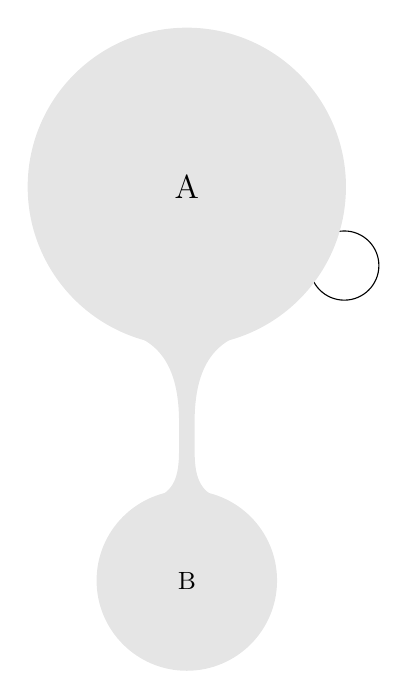
\begin{tikzpicture}
  \node[circle, draw, minimum size=4mm] (q0) {};
  \node[rectangle, draw, right=of q0] (q1) {};
  \node[state] at (2,-1) {};
  \draw[-{Stealth}] (q0) -- (q1);
  \node at ($(q0)!0.5!(q1)$) {};
  \begin{scope}[mindmap, concept color=black!10]
    \node[concept] {A} child {node[concept] {B}};
  \end{scope}
\end{tikzpicture}
\end{document}
